% it/figures/data_pipeline/mode_shapes.tex — versione italiana
\begin{figure}[!ht]
    \centering
    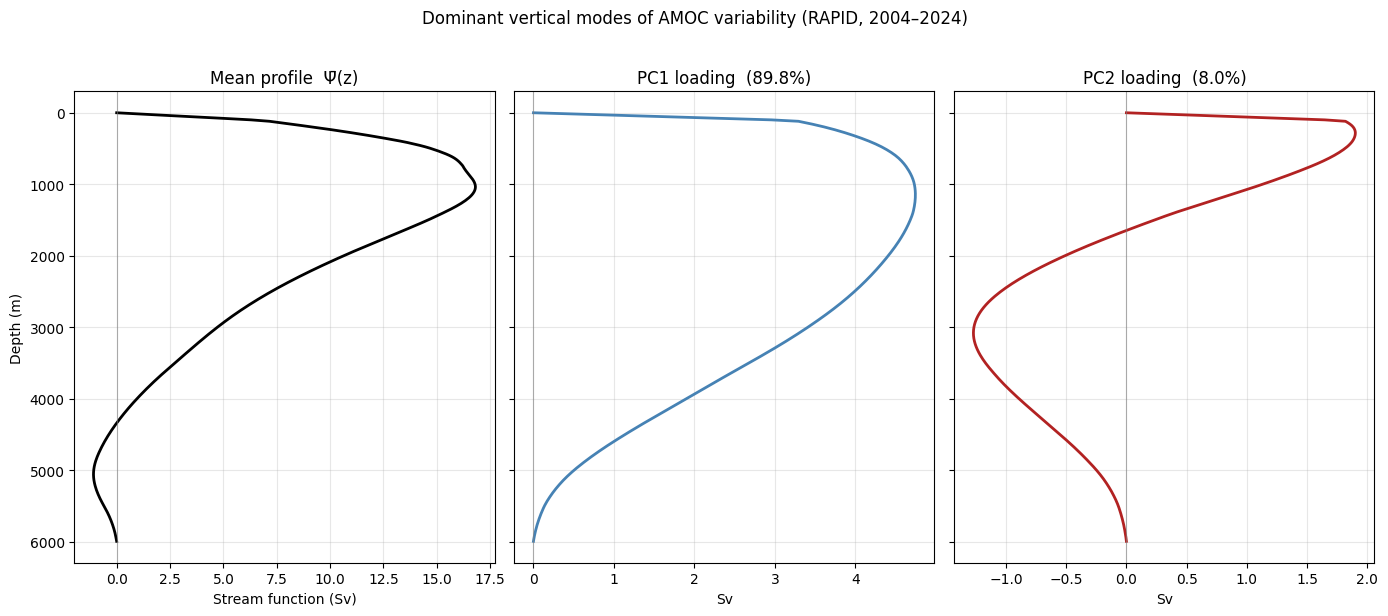
\includegraphics[width=1\textwidth]{figures/data_pipeline/mode_shapes.png}
    \caption[I due modi verticali: intensità e ridistribuzione.]{\textbf{I due
    modi che spiegano l'anatomia verticale dell'AMOC.} Ogni curva è un profilo di
    loading tracciato rispetto alla profondità. La PC1 (intensità) è un \emph{monopolo}:
    lo stesso segno a ogni profondità, con picco attorno a 1150~m, vicino alla profondità
    a cui il profilo medio ha il suo picco, così che un cambiamento nel suo score rafforza
    o indebolisce coerentemente l'intera cella di rovesciamento.
    La PC2 (ridistribuzione) è un \emph{dipolo}: cambia segno una volta con la profondità,
    rafforzando la cella a un livello mentre la indebolisce a un altro. I loading sono
    scalati in Sv per la visualizzazione. Insieme queste due forme portano il
    \SI{97.86}{\percent} della variabilità verticale.}
    \label{fig:mode-shapes}
\end{figure}
